% !TEX encoding = UTF-8 Unicode

\documentclass[a4paper]{article}

\usepackage{color}
\usepackage{url}
% \usepackage[T1]{fontenc} % enable Cyrillic fonts
% \usepackage[utf8]{inputenc} % make weird characters work
\usepackage{graphicx}
\usepackage[unicode]{hyperref}
\hypersetup{colorlinks,citecolor=green,filecolor=green,linkcolor=blue,urlcolor=blue}

% kodiranje teksta ********************************
\usepackage{fontenc}
\usepackage[utf8]{inputenc}
\usepackage[T1]{fontenc}
\usepackage{lmodern}
\usepackage{amsmath}
\usepackage{pgfplots}
% *************************************************

%% *****************************************************************************************
\usepackage[thmmarks,framed]{ntheorem}			% Paket za podrsku za rad sa teoremama
\usepackage{framed}					% Omogucava da se teorema stavi u okvir

\newtheorem{primer}{Primer}[section]

%%%%%%%%%%%%%%%%%%%%%%
\def\figurename{Slika} 
\def\tablename{Tabela}
% *************************************************************************************
\begin{document}
% *************************************************************************************
% *************************************************************************************

\renewcommand\contentsname{Sadržaj}	
\renewcommand{\refname}{Bibliografija}	
\renewcommand{\abstractname}{Abstrakt}

\title{Brojevni sistemi\\ \small{--- škola računara SystemPro --- }}

\author{Nemanja Mićović\\nmicovic@outlook.com}
\date{Oktobar 2015}
\maketitle

\abstract{
Materijal pred Vama nastao je kao deo kursa Računarstva koji sam držao 2015. godine u školi računara za talentovane - SystemPro, i pokriva deo gradiva vezan za brojevne sisteme. Ukoliko je čitalac 
zainteresovan dublje za navedenu tematiku, može pogledati knjigu \cite{mitic_uor}. Takođe bih napomenuo da je tematika kojom ćemo se baviti u ovom tekstu, izuzetno široko dostupna i lepo 
ilustrovana na Veb-u, te svakako preporučujem da pogledate navedeni deo gradiva i tu.
}
\tableofcontents

\newpage

% ************************************************************
\section{Uvod u brojevne sisteme}
\label{sec:uvod}
% ************************************************************
\subsection{Prirodno pitanje o računarima}
Na časovima do sada, govorili smo uopšteno o računarima, i trudili smo se da dođemo do razumevanja njihovog celokupnog rada. Prvi korak koji načinismo na tom putu,
jeste bio da računar podelimo na \emph{hardver} i \emph{softver}, odnosno na fizički deo koji se odnosio na komponente, i apstraktni deo koji se odnosio na programe.

Iz te podele, prirodno nam je proisteklo pitanje o samom načinu zapisa podataka u računarima, i ova skripta će na vrlo jednostavan i ilustrativan način predstaviti odgovor na to pitanje.
Kako bismo došli do odgovora, najpre ćemo se malo pozabaviti brojevima samim po sebi, dok ćemo kasnije naučeno iskoristiti da damo konačan odgovor.

Na kraju poglavlja će biti navedeni primeri za vežbu, i čitalac nije u obavezi da ih uradi, ali neka ima na umu da time podsvesno nanosi sebi duševni bol i nemir.

\subsection{Osnovni pojmovi}
Kako bi načini prvi korak ka prosvetljenju naše duše, potrebno je razjasniti sledeće pojmove:
\begin{itemize}
	\item Brojevni sistem
	\item Osnova brojevnog sistema
	\item Binarni brojevni sistem
	\item Oktalni brojevni sistem
	\item Dekadni brojevni sistem
	\item Heksadekadni (heksadecimalni) brojevni sistem
\end{itemize}

\paragraph{Brojevni sistem}je sistem sa jasno definisanim pravilima za zapis broja po nekoj brojevnoj osnovi.
\paragraph{Binarni brojevni sistem}je brojevni sistem sa osnovom 2 i ciframa iz skupa $\{0,1\}$.
\paragraph{Oktalni brojevni sistem}je brojevni sistem sa osnovom 8 i ciframa iz skupa $\{0,1,2,3,4,5,6,7\}$.
\paragraph{Dekadni brojevni sistem}je brojevni sistem sa osnovom 10 i ciframa iz skupa $\{0,1,2,3,4,5,6,7,8,9\}$.
\paragraph{Heksadekadni brojevni sistem}je brojevni sistem sa osnovom 16 i ciframa iz skupa $\{0,1,2,3,4,5,6,7,8,9, A, B, C, D, E, F\}$.



\subsection{Konverzija u dekadni brojevni sistem}
U navedenom delu, biće prikazane konverzije navedenih brojevnih sistema u nama prirodni, dekadni brojevni sistem. Najpe će biti ilustrovan način za zapis bilo kojeg
broja na osnovu kojeg ćemo razviti način za koverziju navedenih sistema u kasnijem delu.

\subsubsection{Osnovni koncept za zapis broja}
Pogledajmo broj 421 i primetimo da važi jednakost:
\begin{primer}
 $$ (421)_{10} = 4\cdot10^2 + 2\cdot10^1 + 1\cdot10^0 $$
\end{primer}

Takođe, pogledajmo nešto veći broj:
\begin{primer}
 $$ (1234567)_{10} = 1\cdot10^6 + 2\cdot10^5 + 3\cdot10^4 + 4\cdot10^3 + 5\cdot10^2 + 6\cdot10^1 + 7\cdot10^0 $$
\end{primer}

I nešto opštije, ukoliko su $a_1, a_2, ..., a_n$ cifre broja:
\begin{primer}
 $$ (a_1a_2a_3...a_{n-1}a_n)_{10} = a_1\cdot10^{n-1}+a_2\cdot10^{n-2}+a_3\cdot10^{n-3}...+a_{n-1}\cdot10^1+a_n\cdot10^0$$
\end{primer}

Odnosno, neki dati broj možemo zapisati u obliku nekih sabiraka koje dobijamo množenjem cifara sa osnovom broja.
U primerima  1.1, 1.2 i 1.3 smo koristili \emph{dekadnu osnovu} broja, i osnova koju smo koristili bila je 10. Primetimo
da je broj 10 u indeksu ispod zagrade sa leve strane navedenih jednakosti, služio da nam naznači koja je osnova u pitanju.

Naša sledeća opsesija je sledeća, hajde da navedeni princip primenimo na druge brojevne osnove kao što su, 2, 8 i 16.

\subsubsection{Binarni brojevni sistem}
Primetimo da smo u dekadnom brojevnom sistemu imali sledeće cifre: $ \{0, 1, 2, 3, 4, 5, 6, 7, 8, 9\} $, dok ćemo u binarnom
sistemu koristiti osnovu 2, čime ćemo u opticaju imati cifre: $ \{0, 1\} $. 

Sledi prikaz stepena broja dva kao i ilustracija funkcije $f(x)=2^x$ prikazana na slici \ref{fig:exp}. \\\\
$ 2^0 = 1 $ \\
$ 2^1 = 2 $ \\
$ 2^2 = 4 $ \\
$ 2^3 = 8 $ \\ 
$ 2^4 = 16 $ \\
$ 2^5 = 32 $ \\
$ 2^6 = 64 $ \\
$ 2^7 = 128 $ \\
$ 2^8 = 256 $\\
$ 2^9 = 512 $ \\
$ 2^{10} = 1024 $ \\
$ 2^{11} = 2048 $ \\
$ 2^{12} = 4096 $ \\
$ 2^{13} = 8192 $ \\
$ 2^{14} = 16 \ 384 $ \\
$ 2^{15} = 32 \ 768 $ \\
$ 2^{16} = 65 \ 536 $ \\
$ 2^{17} = 131 \ 072$ \\
$ 2^{18} = 262 \ 144$ \\
$ 2^{19} = 524 \ 288$ \\
$ 2^{20} = 1 \ 048 \ 576$ \\
$ ... $ \\
$ 2^{32} = 4 \ 294 \ 967 \ 296$ \\
$ ... $ \\
$ 2^{64} = 18 \ 446 \ 744 \ 073 \ 709 \ 551 \ 616$ \\
$ ... $ \\
$ 2^{95} = 39 \ 614 \ 081 \ 257 \ 132 \ 168 \ 796 \ 771 \ 975 \ 168$ \\

\begin{figure}[h!]
  \begin{center}
    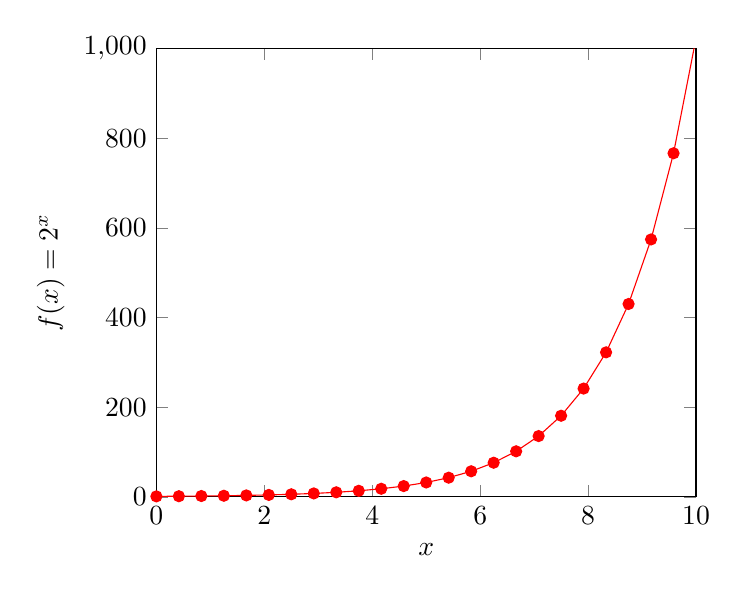
\begin{tikzpicture}
      \begin{axis}[
	xlabel=$x$,
	ylabel={$f(x) = 2^x$},
	ymin=0, ymax=1000,
	xmin=0, xmax=10
      ] 
	\addplot[color=red, domain=0:10,mark=*] {2^x}; 
      \end{axis}
    \end{tikzpicture}
  \caption{Funkcija $f(x) = 2^x$}
  \label{fig:exp}
  \end{center}
\end{figure}

Primetimo da brojevi izuzetno brzo rasto, što je i očekivano, jer su stepeni broja dva podskup eksponencijalne funkcije $f(x)=a^x$, gde je $a=2$, a $x$ iz skupa prirodnih brojeva. 

Navedimo par primera i primenimo ideju ilustrovanu ranije za dekadni brojevni sistem.

\begin{primer}
 $$ (1101)_2 = 1\cdot2^3 + 1\cdot2^2 + 0\cdot2^1 +  1\cdot2^0 
	     = (13)_{10}$$
\end{primer}

\begin{primer}
  $$ (11111)_2 = 1\cdot2^4 + 1\cdot2^3 + 1\cdot2^2 + 1\cdot2^1 +  1\cdot2^0 
	     = (31)_{10}$$
\end{primer}

I naravno opštije :
\begin{primer}
  $$(a_1a_2...a_{n-1}a_n)_2 = a_1\cdot2^{n-1}+a_2\cdot2^{n-2}+...+a_{n-1}\cdot2^{1}+a_n\cdot2^0$$
\end{primer}

Primetimo da možemo na brži način izračunati dekadnu vrednost binarnog broja dopisivanjem odgovorajućih stepena broja dva iznad cifara, od desne strane ka levoj:
\begin{primer}
 $$ \big(\overbrace{1}^{8}\overbrace{1}^{4}\overbrace{0}^{2}\overbrace{1}^{1}\big)_2 = 8 + 4 + 1 = (13)_{10} $$
\end{primer}

\begin{primer}
 $$ \big(\overbrace{1}^{32}\overbrace{0}^{16}\overbrace{1}^{8}\overbrace{1}^{4}\overbrace{1}^{2}\overbrace{0}^{1}\big)_2 = 32 + 8 + 4 + 2 = (46)_{10}$$
\end{primer}

\subsubsection{Oktalni brojevni sistem}
Oktalni sistem je brojevni sistem zasnovan na osnovi 8. Time su cifre koje koristimo: $ \{ 0, 1, 2, 3, 4, 5, 6, 7 \} $. Pokažimo par primera sa konverzijama brojeva i oktalnog sistema u dekadni.

\begin{primer}
 $$ (312)_8 = 3\cdot8^2 + 1\cdot8^1 + 2\cdot8^0 = (201)_{10}$$
\end{primer}

\begin{primer}
 $$ (1373)_8 = 1\cdot8^3+3\cdot8^2+7\cdot8^1+3\cdot8^0 = (761)_{10}$$
\end{primer}

\subsubsection{Heksadekadni brojevni sistem}
Heksadekadni sistem je brojevni sistem zasnovan na osnovi 16. Do sada smo videli dekadni, binarni i oktalni brojevni sistem, i primetili smo da brojevni sistemi koriste cifre od $0$ pa sve do $n-1$, 
gde je $n$ osnova brojevnog sistema. Postavlja se pitanje, kako da reprezentujemo cifre 10, 11, 12, 13, 14 i 15 koje su potrebne za heksadekadni sistem?

Ako je skup cifara dat kao $ \{0,1,2,..,9,10,11,12,13,14,15\} $ ne bismo se usrećili jer bismo izgubili jednoznačnost zapisa. 
Na primer $ (112)_{16} $. Da li je tu 11 cifra, ili je 12 cifra, ili su to cifre 1, 1, 2 ?

Ali ako pokušamo sa $ \{0,1,2...,9,a,b,c,d,e,f \} $, nećemo izgubiti jednoznačnost zapisa, pri čemu novouvedene cifre definišemo kao: \\
$$ A = 10 $$
$$ B = 11 $$
$$ C = 12 $$
$$ D = 13 $$
$$ E = 14 $$
$$ F = 15 $$

Nije važno da li se koriste mala ili velika slova, i u drugim literaturama će se često sresti oba.

\begin{primer}
 $$ (F14)_{16} = 15\cdot16^2+1\cdot16^1+4\cdot16^0 = (3860)_{16}$$
\end{primer}

\begin{primer}
 $$ (CD32)_{16} = 12\cdot16^3+13\cdot16^2+3\cdot16^1+2\cdot16^0 = (52530)_{16}$$
\end{primer}

\subsection{Ostale konverzije}
U ovom delu ćemo prikazati još neke zanimljive načine da obavimo konveziju iz brojevnih sistema u drugi. Posebno je zanimljiv slučaj kada je osnova jednog brojevnog sistema stepen
osnove drugog brojevnog sistema kao što je to slučaj sa binarnim.

Odnosno, osnova binarnog sistema je 2, dok su osnove oktalnog i heksadekadnog, 8 i 16. Primetimo da je $8=2^3$ i $16=2^4$, odnosno da su osnove ova dva sistema, stepeni broja 2. 
Ovo izuzetno olakšava konverziju brojeva u takvim sistemima jer se mogu grupisati cifre na odgovarajući način, i potom se jednostavno pretvoriti u odgovarajuće cifre drugog brojevnog sistema.
Sledeći deo nam pokazuje navedeno kroz primere.

\subsubsection{Konverzija oktalni-binarni}

Neka je dat broj sledeći oktalni broj:
$$ (2471)_8 = (1337)_{10}$$

Primetimo da važi:
$$ \big(\overbrace{2}^{010}\overbrace{4}^{100}\overbrace{7}^{111}\overbrace{1}^{001}\big)_8 $$

Odnosno:
$$ (2471)_8 = (010 \ 100 \ 111 \ 001)_2 = (1337)_{10} $$

Kako izvršiti konverziju unazad? Ideja je slična, uzmemo po tri cifre krećući sa desna, i njih direktno konverzujemo u oktalne cifre.

$$ \big(\overbrace{010}^{2}\overbrace{100}^{4}\overbrace{111}^{7}\overbrace{001}^{1}\big)_2 = (2471)_8 $$

Zašto po 3? Prisetimo se da je $2^3=8$, odnosno sa binarnim brojem dužine 3, možemo predstaviti sve oktalne cifre.

Šta ako je dat binarni broj koji nema dovoljno cifara za naše uparivanje dužine 3. Na primer:
$$ \big(\overbrace{1}^{?}\overbrace{100}^{4}\overbrace{111}^{7}\overbrace{001}^{1}\big)_2 $$

Jednostavno dopunimo nulama sa leve strane:
$$ \big(\overbrace{001}^{1}\overbrace{100}^{4}\overbrace{111}^{7}\overbrace{001}^{1}\big)_2 $$

\subsubsection{Konverzija heksadekadni-binarni}
Logika je slična kao za oktalni sistem, jedino ćemo uzimati 4 cifre umesto 3.

$$ \big(\overbrace{F}^{1111}\overbrace{A}^{1010}\overbrace{3}^{0011}\overbrace{8}^{1000}\big)_{16} = (1111 \ 1010 \ 0011 \ 1000)_2$$

I obrnuto:

$$ \big(\overbrace{1111}^{F}\overbrace{1010}^{A}\overbrace{0011}^{3}\overbrace{1000}^{8}\big)_{16} $$

I naravno, kada ne možemo da uparimo brojeve na odgovarajući način, možemo dopuniti nulama kao kod oktalnog sistema.
$$ \big(\overbrace{10}^{?}\overbrace{1010}^{A}\overbrace{0011}^{3}\overbrace{1000}^{8}\big)_{16} $$
$$ \big(\overbrace{0010}^{2}\overbrace{1010}^{A}\overbrace{0011}^{3}\overbrace{1000}^{8}\big)_{16} $$


% ************************************************************
\section{Reprezentacija podataka u računaru}
\label{sec:data}
% ************************************************************
U poglavlju \ref{sec:uvod} dali smo ilustraciju različitih brojevnih sistema, ali ono što jeste bio najvažniji zaključak za nas, jeste da smo sve prirodne brojeve (odnosno ne baš sve jer ih ima beskonačno) 
mogli da zapišemo kao binarne brojeve. Binarni brojevni sistem je izuzetno važan u svetu računarstva i upravo su binarni brojevi osnova samih računara. 
Ne samo da možemo zapisati sve prirodne brojeve binarno, već možemo zapisati i negativne brojeve, kao i realne. Danas se negativni brojeve zapisuju koristeći \emph{potpuni komplement}, dok se realni
brojevni zapisuju po standardu \emph{IEEE 754} izdatim 1985. No trenutnu nam nije neophodno poznavanje ova dva navedena, te ih ostavljamo za neke bolje dane.

\subsection{Osnovni pojmovi}
Posmatrajmo sledeći binarni broj:
$$ (0011 \ 1100)_2 $$

Razjasnimo najpre terminologiju koja prati računarstvo još od nastanka. \\
\emph{Bit} je jedna binarna cifra u binarnom broju, odnosno dati broj ima 8 bita. \\
\emph{Bajt} je binarni broj koji sadrži 8 bita, odnosno gore navedeni broj je jedan bajt. \\

Primetimo da ako broj ima 32 bita, onda on ima 4 bajta, a ukoliko je 64-bitni, onda ima 8 bajta. Na dalje možemo izvesti sistem
za meru količine podataka na sledeći način (pod B podrazumevamo bajt):

\begin{itemize}
 \item Bajt - B
 \item Kilobajt - KB
 \item Megabajt - MB
 \item Gigabajt - GB
 \item Terabajt - TB
 \item Petabajt - PB
 \item Eksabajt - EB
 \item Zetabajt - ZB
 \item Jotabajt - YB
\end{itemize}

Gde važe jednakosti:

\begin{center}
 1KB = 1024B \\
 1MB = 1024KB \\
 1GB = 1024MB \\
 1TB = 1024GB \\
 1PB = 1024TB \\
 1EB = 1024PB \\
 1ZB = 1024EB \\
 1YB = 1024ZB \\
\end{center}

Danas su uobičajeni hard diskovi kapaciteta od po par terabajta, dok su se pre par godina najčešće sretali hard diskovi veličine od 100 do 500 gigabajta. 

\subsection{Kodiranje karaktera}
Pitanje koje se prirodno javlja, je kako u računaru reprezontovati bilo šta što nije broj (videli smo u poglavlju \ref{sec:uvod} kako to da uradimo)? Odgovor nije komplikovan, i zasniva se na kodiranju.
Kodiranje je proces dodele kodova (brojeva) nekim simbolima koje kasnije umemo da protumačimo na osnovu \emph{kodne tabele} ili \emph{kodne šeme}. 

\subsubsection{Binarni brojevi posmatrani kao kodiranje}
Radi ilustracije koncepta kodiranja, uzmimo binarne brojeve dužine 4 bita i konstruišimo kodnu tabelu na osnovu njih (tabela \ref{tabela_binarni}). 

\begin{table}[h!]
\centering
\begin{tabular}{|l|l|}
\hline
kod & broj \\ \hline
0000 & 0  \\ \hline
0001 & 1  \\ \hline
0010 & 2  \\ \hline
0011 & 3  \\ \hline
0100 & 4  \\ \hline
0101 & 5  \\ \hline
0110 & 6  \\ \hline
0111 & 7  \\ \hline
1000 & 8  \\ \hline
1001 & 9  \\ \hline
1010 & 10 \\ \hline
1011 & 11 \\ \hline
1100 & 12 \\ \hline
1101 & 13 \\ \hline
1110 & 14 \\ \hline
1111 & 15 \\ \hline
\end{tabular}
\caption{Kodna tabela binarnih brojeva}
\label{tabela_binarni}
\end{table}

I vrednosti u drugoj koloni tabele jesu upravo dekadne vrednosti odgovarajućih binarnih brojeva sa kojima smo se bavili u poglavlju \ref{sec:uvod}. 
Primetimo još i da ako bismo u tabeli zamenili brojeve 10, 11, 12, 13, 14 i 15 sa A, B, C, D, E, F dobili bismo direktno kodiranje heksadekadnih brojeva.

Kodne tabele nam olakšavaju kodiranje i dekodiranje simbola jer sve što je potrebno da se učini jeste da se pogledaju odgovarajuća polja u tabeli, i dođe do potrebne informacije. 
Na primer potrebno je da kodiramo broj 13 u binarni broj? Pogledamo tabelu pod broj 13 i vidimo da mu odgovara broj 1101.

\subsubsection{ASCII tabela}
ASCII (engl. \emph{American Standard Code for Information Interchange}) je kodna tabela izdata 1963. godine, i od tada je doživljavala razne dopune i izmene. ASCII je 7-bitni kod kojim 
možemo reprezentovati 128 karaktera. U vreme kada je ASCII izdat, tadašnji računari su uglavnom bili 8-bitni (današnji su 32-bitni i 64-bitni), te se poslednji osmi bit najčešće koristio kao bit parnosti
kojim se proveravala greška u bajtu.

Programski jezik C koristi ASCII tabelu kao osnovnu kodnu šemu za karaktere u svom radu, iako je ASCII tabele za današnje standarde zastarela i mnogo češće se sreću Unicode i UTF-8 kodiranja, koja
dozvoljavaju mnogo širi opseg karaktera koji se mogu kodirati. Slika \ref{fig:ascii_reg} prikazuje jednu ASCII tabelu.

Karakteri kodirani sa:
\begin{itemize}
 \item $[0, 32]$ su kontrolni karakteri
 \item $[48, 57]$ su cifre
 \item $[65, 90]$ su velika slova
 \item $[97, 122]$ su mala slova
\end{itemize}

\begin{primer}
 Neka je dat sledeći kod (dekadni brojevi) koji ćemo protumačiti pomoću ASCII tabele.
 $$ 122 \ 100 \ 114 \ 097 \ 118 \ 111 \ 032 \ 115 \ 118 \ 101 \ 116 \ 101 $$
 
 Primetimo da na osnovu ASCII tabele važe jednakosti: \\
 \begin{center}
  \textsc{122 = z} \\
  \textsc{100 = d} \\ 
  \textsc{114 = r} \\
  \textsc{097 = a} \\ 
  \textsc{118 = v} \\
  \textsc{111 = o} \\
  \textsc{032 = $\_$} \\
  \textsc{115 = s} \\ 
  \textsc{118 = v} \\
  \textsc{101 = e} \\ 
  \textsc{116 = t} \\
  \textsc{101 = e} \\
  \end{center}
  
  Odnosno: \textsc{zdravo svete}
\end{primer}

Naravno, računari rade sa binarnim brojevima, te se ASCII tabela često daje heksadekadno (prisetimo se brzog kodiranja u binarni sistem uzimanjem 4 cifre).

Kodiranje novog reda je zavisno od operativnog sistema, te se novi red kodira na sledeći način:
\begin{itemize}
 \item Windows - CR (Carriage Retrun, kod: 013), LF (Line feed, kod: 010)
 \item Linux - LF
 \item Mac OS X - CR
\end{itemize}


\begin{figure}[h!]
  \begin{center}
    \includegraphics[width=1.0\textwidth]{resources/ascii_regular}
  \end{center}
  \caption{Regularna ASCII tabela}
  \label{fig:ascii_reg}
\end{figure}


% % ************************************************************
% \section{Konverzija brojeva}
% \label{sec:vizija}
% % ************************************************************
% Kao što je pomenuto u uvodu, cilj organizacije KDE jeste delom ono što za cilj i imaju svi Linux projekti - Slobodan softver. Sa druge strane, KDE se vodi i nekim drugim idejama, a ono što čitav
% projekat drži čvrstim i ozbiljnim već dugo jesu sledeća pravila koja važe u KDE zajednici:
% \begin{framed}
%     \begin{itemize}
% 	\item Budite obzirni prema drugima
% 	\item Imajte poštovanja prema drugima
% 	\item Budite otvoreni za saradnju
% 	\item Budite pragmatični
% 	\item Ponudite podršku drugima u zajednici
% 	\item Ne plašite se da zatražite pomoć od zajednice
%     \end{itemize}
% \end{framed}
% 
% Sama zajednica se deli na dva dela i pravila se izuzetno strogo poštuju.
% \begin{itemize}
%  \item Saradnici - učestvuju na razvoju KDE projekta
%  \item Korisnici
% \end{itemize}
% 
% Glavni cilj projekta, oduvek je bio kreirati konzistentan softver udoban za korisnike i tokom godina ta ideja je samo 
% dobijala na snazi te KDE softver danas upravo to i odlikuje - Konzistentan intefejs, izuzetno prijatan za korišćenje 
% kao i kvalitetna sinhronizacija između samih aplikacija što uključuje na primer korišćenje iste teme kroz više 
% tekst editora iako ste je importovali samo u jedan. Više o KDE softver biće reči u poglavlju \ref{sec:softver}.


% ** BIBLIOGRAFIJA **************************************************************
% *******************************************************************************
\newpage
\begin{thebibliography}{9}

\bibitem{mitic_uor}
  Nenad Mitić,
  \emph{Uvod u organizaciju računara},
  Matematički fakultet,
  2009.

\end{thebibliography}
% *******************************************************************************
% *******************************************************************************

%\addcontentsline{toc}{section}{Literatura}
%\appendix
% \bibliography{seminarski} 
% \bibliographystyle{plain}

\end{document}
